\documentclass{article}
\usepackage{amsmath,amssymb}
\usepackage{graphicx}
\usepackage{xcolor}
\usepackage{listings}
\usepackage{fancyhdr}

\pagestyle{fancy}
\fancyhf{}

\rhead{\leftmark}
\fancyfoot[LE,RO]{\thepage}


\renewcommand{\baselinestretch}{1.2}
\setlength{\parskip}{1em}
\definecolor{codegreen}{rgb}{0,0.6,0}
\definecolor{codegray}{rgb}{0.5,0.5,0.5}
\definecolor{codepurple}{rgb}{0.58,0,0.82}
\definecolor{backcolour}{rgb}{0.95,0.95,0.92}

\usepackage{hyperref}
\hypersetup{
    colorlinks,
    citecolor=black,
    filecolor=black,
    linkcolor=black,
    urlcolor=black
}


\lstdefinestyle{mystyle}{
    backgroundcolor=\color{backcolour},   
    commentstyle=\color{codegreen},
    keywordstyle=\color{magenta},
    numberstyle=\tiny\color{codegray},
    basicstyle=\ttfamily\footnotesize,
    breakatwhitespace=false,         
    breaklines=true,                 
    captionpos=b,                    
    keepspaces=true,                 
    numbers=left,                    
    numbersep=5pt,                  
    showspaces=false,                
    showstringspaces=false,
    showtabs=false,                  
    tabsize=2
}

\lstset{style=mystyle}

\begin{document}

\newpage{}
\tableofcontents
\newpage{}

\newpage
\section{Stable Maching problema}

\subsection{Algoritmo Gale-Shapley}
Este algoritmo al terminar de ejecutarse se encuentra un matching prefecto si:
\begin{itemize}
    \item Si existen \(n\) solicitantes con diferentes preferencias.
    \item Si existen \(n\) requeridos con diferentes preferencias.
\end{itemize}
Eligiendo las estructuras correctamente se puede plantear en \(O(n)\).

\begin{lstlisting}[language=Python, caption=Algoritmo de Gale-Shapley]
    Inicialmente M=Vacio
    
    Mientras existe un solicitante sin pareja que no aun se haya postulado a todas las parejas
    
        Sea s un solicitante sin pareja
        Sea r el requerido de su mayor preferencia al que no le
                    solicito previamente
            
        if r esta desocupado
            M = M U (s,r)
            s esta ocupado
        else
            Sea s' tal que (s', r) pertenece a M

            si r prefiere a s sobres s'
                M = M - {(s', r)} U (s,r)
                s esta ocupado
                s' esta libre
    Retornar M
    
\end{lstlisting}    

\newpage
\subsection{Alternativas}
\subsubsection{Diferentes cantidades de oferentes que requeridos}

Dado n oferentes y m requeridos, con \(m <> n\), no se puede encontrar un matching stable. 

Entonces, tenemos que redefinir el concepto de estable. Una pareja (s,r) es \textbf{estable} si:
\begin{itemize}
    \item No existe requerido r' sin pareja al que s prefiera a su actual pareja.
    \item No existe un requerido r' en pareja, tal que s y r' se prefieran sobre sus respectivas parejas.
    \item No existe solicitante s' sin pareja al que r prefiera a su actual pareja.
    \item No existe un solicitante s' en pareja tal que r y s' se prefieran sobre sus respectivas parejas.
\end{itemize}    


Por lo tanto un matching es estable si:
\begin{itemize}
    \item No tienen parejas inestables bajo la condicion anterior.
    \item Que no queden requeridos y solicitantes sin pareja.
\end{itemize}

Soluciones para ajustar al modelo de Gale-Shapley:
\begin{enumerate}
    \item Inventar \(|n-m|\) elementos ficticios
    \begin{itemize}
        \item Los elementos ficticios se pondran en las listas de preferencias con menos elementos.
        \item Estos elementos ficticios se agregan al final y deben ser los menos preferidos.
        \item Luego ejecutar Gale-Shapley
        \item Por ultimo, eliminar las parejas con elementos ficticios. Estos seran los requeridos que quedan sin pareja.
    \end{itemize}
    \item Adecuar el Algoritmo
    \begin{itemize}
        \item Si hay mas \textbf{solicitantes} que requeridos, quitar de la \textit{lista de solicitantes} sin parejas a aquellos que agotaron sus propuestas.
        \item Si hay mas \textbf{requeridos} que solicitantes, quitar de la \textit{lista de parejas} a aquellas donde el requerido quedo sin pareja.
    \end{itemize}
\end{enumerate}

\newpage
\subsubsection{Preferencias incompletas}
Las listas de preferencias de los oferentes y los requeridos son un subset de las contrapartes.

Son parejas \textbf{aceptables} de un elemento a aquellas contrapartes que figuran en su lista de preferencias.

Una pareja (s,r) es \textbf{estable} si:
\begin{itemize}
    \item Son \textit{aceptables} entre ellos.
    \item No existe requerido \textit{aceptable} r' sin pareja al que s prefiera a su actual pareja.
    \item No existe un requerido \textit{aceptable} r' en pareja, tal que s y r' se prefieran sobre sus respectivas parejas.
    \item No existe solicitante \textit{aceptable} s' sin pareja al que r prefiera a su actual pareja.
    \item No existe un solicitante \textit{aceptable} s' en pareja tal que r y s' se prefieran sobre sus respectivas parejas.
\end{itemize}

\begin{quote}
    \textbf{Un matching es estable si no tiene parejas inestables bajo la condicion anterios.}
\end{quote}

\begin{lstlisting}[language=Python, caption=Algoritmo para parejas incompletas]
Inicialmente M=Vacio

#Iterea mientras no haya acotado su sublista de preferencias
Mientras existe un solicitante sin pareja
                'que no aun se haya postulado a todas las parejas' 

    Sea s un solicitante sin pareja
    Sea r el requerido de su mayor preferencia al que no le
                solicito previamente
    
    # se condiera si es aceptable
    if r considera 'aceptable' a s

        if r esta desocupado
            M = M U (s,r)
            s esta ocupado
        else
            Sea s' tal que (s', r) pertenece a M
            si r prefiere a s sobres s'
                M = M - {(s', r)} U (s,r)
                s esta ocupado
                s' esta libre

# Retornar solo parejas aceptables
Retornar M

\end{lstlisting}    


\subsubsection{Preferencias con empates}


\textbf{INDIFERENCIA Y PREFERENCIA ESTRICTA}

\begin{enumerate}
    \item X es \textbf{indiferente} a "y" y a "z" si en su lista de preferencias estan el la misma posicion.
    \item X es \textbf{prefefiere estrictamente} a "y" sobre "z" si en su lista de preferencias no le son indiferentes y 
          "y" se encuentra antes que "z" en la misma.
\end{enumerate}

\noindent
\textbf{ESTABILIDAD DEBIL}
\newline Una pareja (s,r) es debilmente estable si no existe una pareja (s' y r') talque:
\begin{itemize}
    \item s prefiere estrictamente a r' sobre r \textit{(pareja actual de s)}
    \item r' prefiere estrictamente a s sobre s' \textit{(pareja actual de r')}
\end{itemize}



\begin{lstlisting}[language=Python, caption=Algoritmo para parejas incompletas]
    Inicialmente M=Vacio
    
    #Iterea mientras no haya acotado su sublista de preferencias
    Mientras existe un solicitante sin pareja
                    'que no aun se haya postulado a todas las parejas' 
    
        Sea s un solicitante sin pareja
        Sea r el requerido de su mayor preferencia al que no le
                    solicito previamente
            
        if r esta desocupado
            M = M U (s,r)
            s esta ocupado
        else
            Sea s' tal que (s', r) pertenece a M

            # prefiere estrictamente
            si r prefiere estrictamente a s sobres s'
                M = M - {(s', r)} U (s,r)
                s esta ocupado
                s' esta libre
    
    Retornar M
    
\end{lstlisting}    
\begin{quote}
    En caso de que sea empate, se mantendra con su pareja actual.
\end{quote}

\noindent
\textbf{ESTABILIDAD FUERTE}
\newline Una pareja (s,r) es debilmente estable si no existe una pareja (s' y r') talque:
\begin{itemize}
    \item s prefiere estrictamente o le es indiferente a r' sobre r \textit{(pareja actual de s)}
    \item r' prefiere estrictamente o le es indiferente a s sobre s' \textit{(pareja actual de r')}
\end{itemize}
Puede no existir un matching perfecto.

\begin{lstlisting}[language=Python, caption=Algoritmo para parejas super estables]
    Inicialmente M=Vacio
    
    Mientras existe un solicitante sin pareja y no exista solicitante que agoto sus parejas
    
        Sea s un solicitante sin pareja
        Sea r el requerido de su mayor preferencia al que pueda proponer
        Por cada sucesor s' a s en la lista de preferencias de r
            if (s',r) pertence a M
                M = M - {(s',r)}
                s' esta libre
            quitar s' de la lista de preferencias de r
            quitar r de la lista de preferncias de s'

        Por cada requerido r' que tiene multiples parejas
            Por cada pareja s' en pareja con r' 
                M = M - {(s',r')}
                quitar s' de la lista de preferencias de r'
                quitar r' de la lista de preferencias de s'

    if estan todos en pareja
        Retornar M
    else
        No existe ningun matching super estable
\end{lstlisting}    
\begin{quote}
    En caso de que sea empate, se mantendra con su pareja actual.
\end{quote}

\newpage
\subsubsection{Agrupacion de 1 a muchos}
El solicitante puede tener varios cupos por lo tanto:
\begin{itemize}
    \item Exiten \(m\) requeridos, donde un requerido puede estar unicamente con 1 pareja.
    \item Exiten \(n\) solicitantes, donde cada solicitante puede tener \(c\) cupos para armar parejas.
\end{itemize}

Existe un matching estable si la cantidad de requeridos es igual a la cantidad de solicitantes por la cantidad de cupos.

\begin{equation} \label{eu_eqn}
    m=n*c
\end{equation}

No cambia la definición de Gale Shampey para \textbf{matching estable}

\begin{lstlisting}[language=Python, caption=Algoritmo de solicitantes con cupos]
    Inicialmente M=Vacio
    
    Mientras exista un solicitante con cupo disponible
    
        Sea s un solicitante sin pareja
        Sea r el requerido de su mayor preferencia al que no le
                    solicito previamente
            
        if r esta desocupado
            M = M U (s,r)
            s decremente su disponibilidad de parejas
        else
            Sea s' tal que (s', r) pertenece a M

            si r prefiere a s sobres s'
                M = M - {(s', r)} U (s,r)
                s decremente su disponibilidad de parejas
                s' incrementa su disponibilidad de parejas
    Retornar M
    
\end{lstlisting}    
\begin{quote}
    \textbf{La complejidad algoritmica no se modifica porque solo se agrega un contador.}
\end{quote}

\newpage
\subsubsection{Agrupacion de muchos a 1}
El requerido puede tener varios cupos por lo tanto:
\begin{itemize}
    \item Exiten \(m\) requeridos, donde cada solicitante puede tener \(z\) cupos para armar parejas.
    \item Exiten \(n\) solicitantes, donde un requerido puede estar unicamente con 1 pareja.
\end{itemize}

Existe un matching estable si la cantidad de solicitantes es igual a la cantidad de requeridos por la cantidad de cupos.

\begin{equation} \label{eu_eqn}
    n=m*z
\end{equation}

No cambia la definición de Gale Shampey para \textbf{matching estable}

\begin{lstlisting}[language=Python, caption=Algoritmo de requeridos con cupos]
    Inicialmente M=Vacio
    
    Mientras exista un solicitante con cupo disponible
    
        Sea s un solicitante sin pareja
        Sea r el requerido de su mayor preferencia al que no le
                    solicito previamente
            
        if r tiene cupo 
            M = M U (s,r)
            s esta ocupado
            r decrementa su disponibilidad de parejas
        else
            Sea s' tal que (s', r) pertenece a M y 
                    s' es el menos preferidos de las parejas r

            si r prefiere a s sobres s'
                M = M - {(s', r)} U (s,r)
                s esta ocupado
                s' esta libre
    Retornar M
    
\end{lstlisting}    
\begin{quote}
    \textbf{La complejidad algoritmica si se modifica.}
\end{quote}
Para conocer el solicitante de menor preferencia podemos utilizar un heap de minimos. Como el cupo es de z, la complejidad algoritmica para actualizar el heap es \(log (z)\).

\newpage
\subsubsection{Agrupacion de y a x}
\begin{itemize}
    \item Exiten \(n\) solicitantes, donde cada solicitante puede tener \(c\) cupos para armar parejas.
    \item Exiten \(m\) requeridos, donde cada requerido puede tener \(z\) cupos para armar parejas.
\end{itemize}


Existe un matching estable si:

\begin{equation} \label{eu_eqn}
    n*c=m*z
\end{equation}


No cambia la definición de Gale Shampey para \textbf{matching estable}
\newline
Para implementar se requieren las siguientes estructuras:
\begin{itemize}
    \item Un heap de minimos para los requeridos.
    \item Un contador de cupos para los solicitantes.
\end{itemize}

\begin{quote}
    \textbf{La complejidad algoritmica es igual a la de los requeridos con cupos}
\end{quote}

\newpage
\subsubsection{Conjuntos no bipartios - Stable Roommate Problem}
Pendiente

\newpage
\section{Analisis amortizado}

\subsubsection{Metodo de agregacion}
\subsubsection{Metodo del banquero}
\subsubsection{Metodo del potencial}

\newpage
\subsubsection{Heap binomial y fibonacci}
Revisar capitulo 19 del Corven.
\newline
Para el \textbf{heap binomial} se utilizan bosques de arboles binarios. Existe un proceso donde se van ordenando los arboles.

Al insertar, se parece al ejemplo de contador binario y la amortizacion es O(1)
\newline
Decrementar en un log binomial, es log(n) porque no es posible amortizar
\newline 
Eliminar el minimo, es el el peor caso es log(n)

Para el \textbf{heap fibonacci} ...

\section{Algoritmos Greedy}

Utiliza heurisica de seleccion para encontrar una solución global optima despues de muchos pasos.

\subsection{Mochila fraccionaria}

Dado un contener de capacidad W, y un conjunto de elementos n fraccionables de valor \(v_i\) y peso \(w_i\)

El objetivo es seleccionar un subconjunto de elemento o fracciones de ellos de modo de maximizar el valor almacenado y sin superar la capacidad de la mochila.

La complejidad es \(O(nlog(n))\)

\newpage
\subsection{Cambio de moneda}

Es una solución es conocido como solución de cajero. Contamos con un conjunto de diferentes monedas de diferentes denominación sin restricción de cantidad.

\[
    \$=(C_1,C_2,C_3,\cdots,C_n)  
\]

El objetivo es entregar la menor cantidad posible de monedas como cambio.

Tiene una complejidad de \(O(n)\).

El sistema \(\$\) se conoce como \textbf{canonico} a aquel en el que para todo x, \(greedy(\$,x)=optimo(\$,x)\).

Para saber si una base es canonica:
\begin{enumerate}
    \item Basta con buscar un contraejemplo. Estaria entre la 3ra denomininacion y la suma de las ultimas dos doniminaciones.
    \item Utilizar un algoritmo Polinimico para determinar si es un sistema canonico.
\end{enumerate}

Si el problema no es greddy, se puede construir un algoritmo utilizando programación dinamica.


\newpage
\subsection{Interval Scheduling: Algoritmo de Greedy Stay Ahead}

Tenemos un conjunto de requests \(\{1,2,..,n\}\); el request \(i^{th}\) corresponde a un intervalo de tiempo que comienza al instante \(s(i)\) y finaliza al instante \(f(i)\).
Diremos que un subconjunto de requests es compatible si no hay dos de ellos que al mismo tiempo se superponen, y nuestro objetivo es aceptar un subconjunto compatible tan grande como sea posible. El conjunto compatible con mayor tamaño sera el \textbf{óptimo}.

La idea básica en un algoritmo greedy para interval scheduling es usar una simple regla para seleccionar el primer request \(i_1\). Una vez que el request \(i_1\) aceptado, rechazamos todos los request que no son compatibles con \(i_1\). Luego seleccionamos el siguiente request \(i_2\), y volvemos a rechazar todos lo request que no son compatibles con \(i_2\). 
Continuamos de esta manera hasta que nos quedemos sin requests. El desafio en diseñar un buen algoritmo greedy esta en decidir que regla usar para la selección.

Pueden probar con varias reglas, pero las mas optimo es la siguiente idea: Aceptaremos el request que termina primero, o sea el request para el cual tiene el menor \(f(i)\) posible. 
Asi nos aseguramos que nuestros recursos se liberen tan pronto como sea posible mientras satisfacemos un request. De esta manera podemos maximizar el tiempo restante para satisfacer otro request.

Para escribir el pseudo código, utilizaremos \(R\) para denotar al conjunto de request que aún no estan aceptados ni rechazados, y usaremos \(A\) para denotar al conjunto de los request aceptados.

\begin{lstlisting}[language=Python, caption=Algoritmo de greedy para Interval Scheduling]
Inicialmente R contiene todos los requests, y A es un conjunto vacio.

Mientras R no esta vacio

    Seleccionar un request i de R que tenga el instante de finalizacion mas chico.
    Agregar el registro i a A
    Eliminar todos los request de R que no sean compatibles con el request i    

Fin mientras

Retornar el conjunto A como el conjunto de los request aceptados.

\end{lstlisting}    


\begin{figure}[h!]
    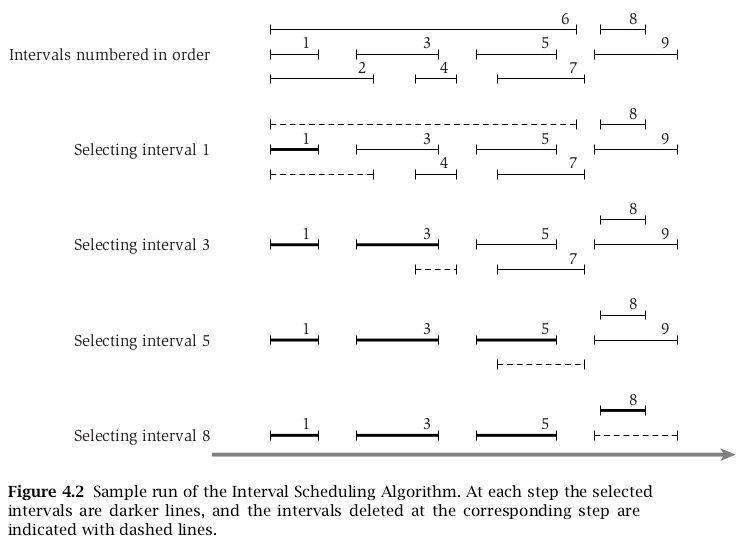
\includegraphics[width=\linewidth]{imagenes/intervalos-compatibles.png}
\end{figure}

\begin{quote}
    De forma inmediata podemos decir que el conjunto retornado tiene request compatibles.
\end{quote}

Lo que necesitamos es demostrar que la solución es optima. Definimos a \(O\), un conjunto de intervalos optimos. 
Luego, vamos a mostrar que \(|A| = |O|\), o sea que el conjunto \(A\) tiene la misma cantidad de intervalos que \(O\), y por lo tanto, \(A\) tambien es una solución optima.

Para la prueba introduciremos la siguiente notación:
\begin{itemize}
    \item Dado \(\{i_1,...,i_k\}\) el conjunto de request en \(A\) en orden que fueron agregados a \(A\). Notar que \(|A|=k\).
    \item Dado \(\{j_1,...,j_m\}\) el conjunto de request en \(O\) ordenos de izquierda a derecha. Notar que \(|O|=m\).
\end{itemize}
El objetivo es probar que \(k=m\).

La manera en que el algoritmo de greedy se mantenga adelante(\textbf{stays ahead}) es que cada uno de sus intervalos finalice al menos tan pronto como lo haga el correspondiente intervalo en el conjunto \(O\).

\begin{figure}[h!]
    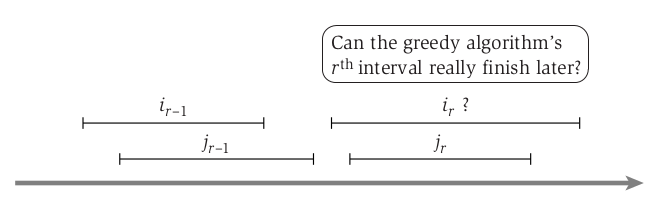
\includegraphics[width=\linewidth]{imagenes/demo-greedy-intervalos.png}
\end{figure}

\begin{quote}
    \textbf{(3.1) Para todos los indices \(r<k\) tenemos que \(f(i_r) \leq f(j_r)\)}
\end{quote}

\textbf{Demostración:}  Probaremos la sentencia anterior mediante el método inductivo. Para \(r=1\) la sentencia anterior es cierta, el algoritmo empieza seleccionando el request \(i_1\) con el menor tiempo de finalización.

Para el caso inductivo, o sea \(r>1\) asumiremos como nuestra hipotesis inductiva que la sentencia es verdadera para \(r-1\), y queremos probar que es tambien es lo es para \(r\). La hipotesis inductiva nos dice que asumamos verdadero que \(f(i_{r-1}) \leq f(j_{r-1})\). Queremos demostrar que \(f(i_{r}) \leq f(j_{r})\).

Dado que \(O\) consiste en intervalos compatibles, sabemos que \(f(j_{r-1}) \leq s(j_r)\). Combinando esto último con la hipotesis inductiva \(f(i_{r-1}) \leq f(j_{r-1})\), obtenemos \(f(i_{r-1}) \leq s(j_{r})\). Asi el intervalo \(j_r\) esta en conjunto \(R\) de los intervalos disponibles al mismo tiempo cuando el algoritmo de greedy selecciona \(i_r\).
El algoritmo de greedy selecciona el intervalo con el \textit{tiempo final mas chico} (\(i_{r}\)); y dado que intervalo \(j_{r}\) es uno de estos intervalos, tenemos que \(f(i_r) \leq f(j_r)\), completando asi el paso inductivo.

De esta forma demostramos que nuestro algoritmo se mantiene adelante del conjunto optimo \(O\). Ahora veremos porque esto implica optimalidad del conjunto \(A\) de algoritmo de greedy.

\begin{quote}
    \textbf{El algoritmo de greedy retorna un conjunto \(A\) óptimo.}
\end{quote}

\textbf{Demostración:} Para demostrarlo utilizaremos la contradicción. Si \(A\) no es optimo, entonces el conjunto \(O\) debe tener mas requests, o sea que tenemos \(m>k\) y aplicando 3.1, cuando r=k, 
obtenemos que \(f(i_k) \leq f(j_k)\). Dado que \(m>k\), existe un request \(j_{k+1}\) en \(O\). Este request empieza despues que el request \(j_k\) termina y por consiguiente despues de que el request \(i_k\) termine.
Entonces, despues de eliminar todos los requests que no son compatibles con los request \(i_1,...,i_k\), el conjunto de posibles requests R aún contiene el requests \(j_{k+1}\). 
Pero el algoritmo de greedy se detiene con el request \(i_k\) y este supuestamente se detiene porque \(R\) esta vacio, lo cual es una contradicción. 


\newpage
\subsection{Seam Carving - TODO}
Es un algoritmo para adecuar imagenes. Analiza imagenes recortando pixeles de menor importancia. Retira tantas vetas como sea necesario para llegar a un tamaño optimo.


\subsection{Caminimos Minimos - TODO}

Dado dos nodos, uno inicial \(s\) y otro final \(t\) el algoritmo encuentra el camino minimo que los une, tambien entre \(s\) y el resto de los nodos.

\subsection{Compresión de datos - TODO}

El algoritmo de greedy arma un arbol de "hufman" para armar un arbol optimo de prefijos.

\section{División y conquista}

\subsection{Teorema mestro - TODO}


\subsection{Mediana con datos separadas}




\newpage
\section{Programación dinamica}

\subsection{Cambio de monedas}

Contamos con un conjunto de monedas de diferente denominación sin restricción de cantidad. 
Representamos de esta manera \(\$=(c_1,c_2,....,c_n)\) y tenemos un importe \(x\) a dar. 
Concluimos que no existe un algoritmo satisfactorio de greedy para resolver este problema.

Si buscamos la solución por \textbf{fuerza bruta}, se puede armar un arbol de decisión. 
Por cada moneda posible, se genera un subproblema. 

\begin{figure}[h!]
    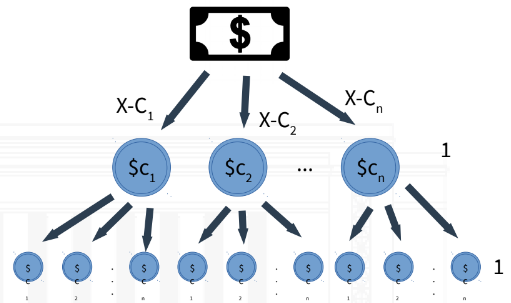
\includegraphics[width=\linewidth]{imagenes/dinamico-arbol-moneda.png}
\end{figure}

Entonces el camino a la hoja con menor profundidad es la menor cantidad de monedas a dar. Esto hace que la complejidad sea \(O(x^n)\).

Analizando el problema anteriores se pueden obtener algunas mejoras. 
Parte de los caminos del arbol son iguales. 
Hay distintas ramas con nodos que tienen el mismo resto, 
y por lo tanto se puede calcular solo una vez. 
Este caso de resto igual en varios nodos, lo llamaremos subproblemas.

\begin{figure}[h!]
    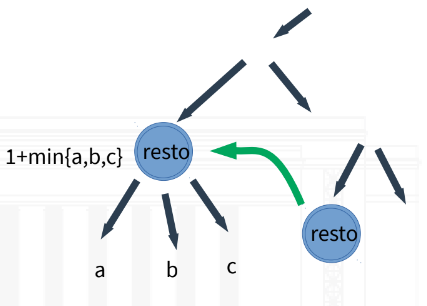
\includegraphics[scale=0.5]{imagenes/dinamico-moneda-subproblema.png}
\end{figure}

\newpage
\textbf{Subproblema}: Calcular el óptimo(OPT) del cambio \(x\) debe usar el mínimo entre los subproblemas \(X - C_j\) para \(j=1...n\).

Cada vez que paso por un subproblema se incremente en \(1\) para contar la cantidad de monedas a dar. 
Que seria: \(1+min\{subproblemas\}\).

Para la solución \textbf{recurrente}, podemos plantear:

    \[
        \left\{ \begin{array}{lcc}
            OPT(x) = 0 &   si  & x = 0 \\
            \\ OPT(x) = 1+min\{OPT(x-C_i)\} &  si & x > 0 \\
            \end{array}
        \right.
    \]

El resultado con el minimo cambio sera OPT(x) y para poder calcularlo, 
necesito calcular los \(x-1\) óptimos anterios. 
Para evitar el recalculo, si calculo el optimo de algun resto, 
lo almaceno para no volver a calcularlo de nuevo.
Ademas en cada subproblema debo analizar \(n\) comparaciones, lo cual impacta en la complejidad.

\noindent
\underline{SOLUCIÓN ITERATIVA}
\begin{lstlisting}[language=Python, caption=Solución iterativa]

OPT[0] = 0
Desde i=1 a X
    minimo = +infinito
    Desde j=1 a n
        resto = i - C[j]
        si resto > 0 y minimo > OPT[resto]
            minimo = OPT[resto]
    
    OPT[i] = 1 + minimo

Retornar OPT[X]
\end{lstlisting}

La complejidad es \(O(X*n)\) porque no solo depende de los diferentes tipos de monedas, tambien
depende del parametro de entrada \(X\). Se dice que es un algotimo pseudo polinomial.

\noindent
\underline{RECONSTRUIR LAS ELECCIONES}

\begin{lstlisting}[language=Python, caption=Solución iterativa con reconstrucción]

OPT[0] = 0
elegida[0] = 0
Desde i=1 a X
    minimo = +infinito
    elegida[i] = 0
    Desde j=1 a n
        resto = i - C[j]
        si resto > 0 y minimo > OPT[resto]
            elegida[i] = j
            minimo = OPT[resto]
    
    OPT[i] = 1 + minimo

resto = x
Mientras resto > 0
    Imprimir C[elegida[resto]]
    resto = resto - C[elegida[resto]]

Imprimir OPT[x]

\end{lstlisting}

\newpage
\subsection{Problema de la Publicidad en la carretera}

Sea una carretera de longitud \(M\) km, un conjunto de \(n\) carteles publicitarios en el 
intevalo \([0,M]\), cada cartel \(i\) tiene una posición \(x_i\) y un valor de ganancia \(r_i\).
Entonces queremos seleccionar carteles para maximizar la ganancia. Como restriccción ningún cartel
puede estar a menos de 5 km de otro.

\begin{figure}[h!]
    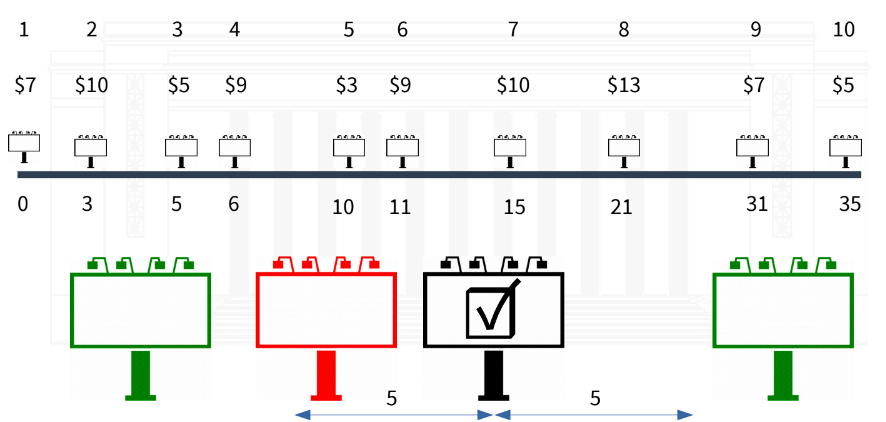
\includegraphics[scale=0.4]{imagenes/dinamico-ejemplo-ruta.png}
\end{figure}

Podemos armar un arbol de decisión utilizando una funcion de \textit{anteriores(i)}. La función anterior
nos dice cual es el cartel anterior al \(i\) que cumple con la restriccción.

\begin{figure}[h!]
    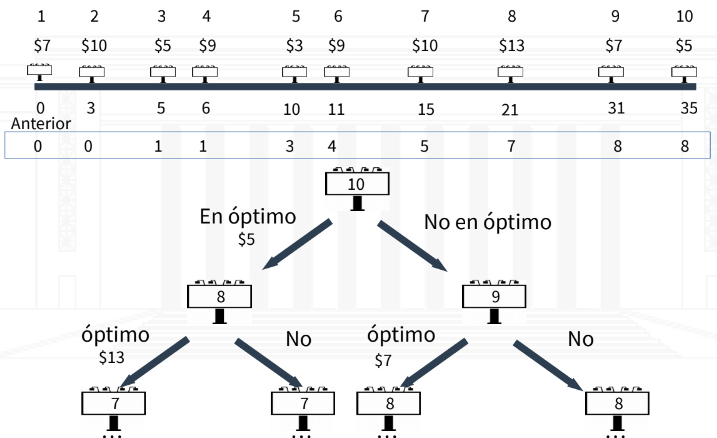
\includegraphics[scale=0.4]{imagenes/dinamico-ruta-arbol.png}
\end{figure}


Para la solución \textbf{recurrente}, podemos plantear:

\[
    \left\{ \begin{array}{lcc}
        OPT(i) = 0 &   si  & i = 0 \\
        \\ OPT(i) = max\{r_i + OPT(anterior(i)), OPT(i-1) \} &  si & i > 0 \\
        \end{array}
    \right.
\]

El resultado con la máxima ganancia sera: \(OPT(n)\). 

\noindent
\textbf{\underline{SOLUCIÓN ITERATIVA}}

\begin{lstlisting}[language=Python, caption=Solución iterativa]

OPT[0] = 0
OPT[1] = r[1]

Desde i=2 a n

    estaCartel = r[i] + OPT[anterior(i)]
    noEstaCartel = OPT[i-1]

    OPT[i] = max (estaCartel, noEstaCartel)

Retornar OPT[n]
\end{lstlisting}


\noindent
\textbf{\underline{SOLUCIÓN ITERATIVA - CARTELES SELECCIONADOS}}

\begin{lstlisting}[language=Python, caption=Solución iterativa con reconstrucción]

OPT[0] = 0
OPT[1] = r[1]
elegidos[0] = false
elegidos[1] = true

Desde i=2 a n

    estaCartel = r[i] + OPT[anterior(i)]
    noEstaCartel = OPT[i-1]

    Si estaCartel>noEstaCartel 
        elegido[i] = true
    sino
        elegido[i] = false

    OPT[i] = max (estaCartel, noEstaCartel)

Retornar OPT[n]
\end{lstlisting}


La complejidad temportal es \(O(n)\) ya que solo hago sumas y comparaciones. La complejidad espacial
es \(O(n)\) porque se almacenan los \(n\) óptimos en un array.

\noindent
\textbf{\underline{SOLUCIÓN ITERATIVA - RECONSTRUIR}}

\begin{lstlisting}[language=Python, caption=Solución iterativa]

i = n

Mientras i>0
    si elegido[i]
        Imprimir i
        i = anterior[i]
    sino 
        i = i-1

Retornar OPT[n]
\end{lstlisting}


La complejidad temportal es \(O(n)\). La complejidad espacial es \(O(n)\).



\noindent
\textbf{\underline{CALCULO CONSTRUIR}}

Se hace un apareo entre las posiciones del cartel \(x\) y el limite del mismo.

\begin{lstlisting}[language=Python, caption=Solución iterativa]

i=n
j=n-1

Mientras i>1
    Si limite(n) >= posicion(j)
        anterior[i] = j
        i=i-1
    sino
        j=j-1

\end{lstlisting}



\newpage
\subsection{Programación de intervalos ponderados}


\newpage
\subsection{Problema de Knapsack (mochila) }

\newpage
\subsection{Problema de Subset Sum }

Sea un conjunto de \(n\) elementos \(E=\{e_1, e_2, ..., e_n \}\) donde cada elemento \(e_i\) 
cuenta con un peso asociado \(w_i\).

Queremos seleccionar un subset de elementos de E con el mayor peso posible que no supere un 
valor \(W\) de peso máximo.

Para plantear una solución por \textbf{fuerza bruta}, un elemento puede estar o no. O sea que si
tengo \(n\) elementos pueden existir \(2^n\) combinaciones. Entonces la complejidad total esta acotado
por \(O(2^n)\).



\newpage
\subsection{Bellman Ford}

Se extiendo el problema de hallar caminos minimos utilizando \textbf{aristas ponderas negativas}. 
Se puede hayar un camino global que pase por aristas ponderadas negativamente y que sea el optimo, 
en vez de utilizar un algotimo de reedy de \textit{Dijkstra} que para este caso no seria óptimo.

Una solución por \textbf{fuerza bruta} seria, calcular para un grafo poderado \textbf{sin ciclos negativos}:

\begin{itemize}
    \item Todos los costos de los caminos posibles de \(s\) a \(t\) de longitud 1.
    \item Todos los costos de los caminos posibles de \(s\) a \(t\) de longitud 2.
    \item ...
    \item Todos los costos de los caminos posibles de \(s\) a \(t\) de longitud n-1.
\end{itemize}

\textbf{El camino mínimo tendra longitud n-1 como máximo} sin ciclos negativos.

El algoritmo de \textbf{Bellman-Ford} halla el camino mínimo con aristas negativos utilizando programación dinámica.

\underline{ANÁLISIS}

Para llegar desde "s" a un nodo \(n_i\) puede haber utilizado diferntes caminino y longitudes.
Lo puede hacer a travez de sus nodos predecesores \(pre[n_i]\).

Para poder llegar a \(n_i\) en \(j\) pasos, tengo que haber llegado a sus predeceroes en \(j-1\) pasos. 
Asi sucesivamente hasta "s" se puede ir resolviendo \textit{sub casos}.

Definimos \(minPath(n,j)\) al camino mínimo hasta el nodo \(n_i\) con longitud máxima \(j\).

\underline{SOLUCIÓN RECURRENTE}

\begin{align*}
minPath('s', j) &= 0 \\
minPath(n_i, 0) &= +\infty & n_i \neq s \\
minPath(n_i, j) &=min\left\{\begin{array}{ll}
                minPath(n_i, j-1)              \\
                min \{minPath(n_x, j-1) + w(n_x, n_i)\}          
        \end{array}\right. & n_x \in pred(n_i)
\end{align*}

\begin{itemize}
    \item El camino mínimo a 's' para cualquier longitud es siempre 0.
    \item El camino mínimo a \(n_i\) al comienzo es infinito.
    \item TODO
\end{itemize}

\underline{SOLUCIÓN ITERATIVA}

Definimos a \(OPT[l][v]\) como el camino mínimo de "s" al nodo \(n\) con longitud\(l\)

El nodo "s" se encuentra en v=0
El nodo "t" se encuentra en v=n

\begin{lstlisting}[language=Python, caption=Algoritmo de requeridos con cupos]
    Desde l=0 a n-1
        OPT[l][0] = 0
    Desde v=0 a n-1
        OPT[0][v] = +infinito


    Desde l=1 a n-1   // max longitud del camino
        Desde v=1 a n // nodo
            OPT[l][v] = OPT[l-1][v]
            Por cada p predecesor de v
                si OPT[l][v] > OPT[l-1][p] + w(p,v)
                    OPT[l][v] = OPT[l-1][p] + w(p,v)
                   
    retornar OPT[n-1, n]
\end{lstlisting}

La complejidad del primer loop esta acotado por n. La segunda parte se ejecuta m veces por cada predecesor.
O sea es \(O(m*n)\)

La complejidad espacial es m*n porque la matriz ocupa n*m

\underline{RECONSTRUIR LAS ELECCIONES}

Agregar un nodo predecesor y almacenar en la posición \(i\) cual fue el predecesor del nodo.

\textit{¿Que pasa si hay un ciclo negativo?}

Si en una iteración despues de haber llegado a la longitud maxima, cambia el minimo de al menos un nodo, entonces el grafo \textit{tiene ciclos negativos}.

\newpage
\subsection{Problema de Maximo subarreglo}

Se necesita calcular un subconjunto \textit{contiguo de elementos} \(S\) 
tal que la suma de los valores sea la máxima posible. 

El maximo subvector que termina en el elemento \(i\), esta relacionado con el máximo
subvector que termina en el elemento \(i-1\).

\underline{SOLUCIÓN RECURRENTE}

\begin{align*}
    MAX(1) &= v[1] \\
    MAX(i) &= max\{MAX(i-1), 0\} + v[i]
\end{align*}
    

\underline{SOLUCIÓN ITERATIVA}

\begin{lstlisting}[language=Python, caption=Solución iterativa]

    MaximoGlobal = v[1]
    MaximoLocal = v[1]
    IdxFinMaximo = 1

    Desde i=2 a n
        MaximoLocal = max(MaximoLocal, 0) + v[i]

        si MaximoLocal > MaximoGlobal
            MaximoGlobal = MaximoLocal 
            IdxFinMaximo = i

    Retornar MaximoGlobal

\end{lstlisting}

\newpage
\subsection{Problema de cuadrados minimos}

Dado un conjunto de puntos \(P={(x_1,y_1),(x_2,y_2),...,(x_n,y_n)}\), con \(x_1<x_2<\cdots<x_n\). 
Usamos \(p_i\) para indicar un punto \((x_i, y_i)\). 

Queremos aproximimar mediante segmentos los puntos de \(P\) minimizando el error comentido. 
Los sementos se forman mediante \textit{rectas de aproximación} hallando \(a\) y \(b\). 
El calculo del error cometido se obtiene sumando las distancias de los puntos a las rectas. 

Se agrega un parametro de penalización \(C>0\) por cada segmento que se agrega.
\begin{itemize}
    \item A mayor "C" entonces: menos segmentos
    \item A menor "C" entonces: menos error
\end{itemize}

Al analizar una solución por \textbf{fuerza bruta} se obtiene una complejidad de \(O(2^{n*n})\).

\underline{SOLUCIÓN RECURRENTE}

Como no conocemos cual es el ultimo segmento, se elige el último segmento como aquel que \textbf{minimice el error general}.  
O sea que queremos minimizar el error del segmento, mas la constante \(c\) 
mas el error conocido en el \textit{subproblema que contiene los puntos de segmentemos anteriores} 
sea el minimo entre todos los posibles.


\begin{align*}
    OPT(i) &= min_{1 \leq x \leq i} (e_{x,i} + C + OPT(x-1)) \\ 
    OPT(0) &= 0
\end{align*}
    
\noindent
\underline{SOLUCIÓN ITERATIVA}

\begin{lstlisting}[language=Python, caption=Solución iterativa]
    OPT[0] = 0

    Para todo para i,j con i <= j
        Calcular e[i][j]

    Desde j=1 a n
        OPTIMO[j] = +infinito
    
        Desde i=1 a n
            segmento = e[i][j] + C + OPT[i-1]

            si OPTIMO[j] > segmento 
                OPTIMO[j] = segmento

    Retornar OPT[n]

\end{lstlisting}

Analizando la \textbf{complejidad temporal}, el calculo del optimo es \(O(n)\), pero se calculan \(n\) óptimos,
Por lo tanto esta partes es \(O(n^2)\).

Pero como en la primer se itera sobre todos los pares posibles es \(O(n)\). Y como el calculo del error
es \(O(n)\), la primer interación termina siendo \(O(n^3)\), y este le gana a \(O(n^2)\).

La complejidad total es \(O(n^3)\).

Para el calculo de la \textbf{complejidad espacial}, los errores se almacenan en \(O(n^2)\), mientras que 
los óptimos en \(O(n)\). Por lo tanto la complejidad espacial total es de \(O(n^2)\).

\newpage
\subsection{Problema del viajante}

Sea un conjunto de \(n\) ciudades "C", un conjunto de rutas de costo de tránsito, existe una ruta 
que une cada par de ciudades.

Queremos obtener el circuito de menor costo que inicie y finalice en una ciudad y
que pase por el resto de las ciudades \textit{una y solo una} vez

Mediante \textbf{fuerza bruta} tenemos que calcular todos los ciclos posibles, y por lo tanto
existen \((n-1)!\) ciclos de longitud \(n-1\). 
Luego por cada ciclo calculamos su costo y nos quedamos con el mínimo. Por lo tanto la complejidad total es \(O(n!)\).

Mediante el \textbf{algoritmo Belman-Held-Karp} lo resuelvo utilizando programación dinamica.
Se puede decomponer como el mínimo entre los subproblemas menores con \((n-1)!\) hojas.

\noindent
\underline{SOLUCIÓN RECURRENTE}

Dado \(S\) un subconjunto de ciudades e \(i\) la ciudad donde estoy parado. \textbf{start} es la ciudad de partida.
La siguiente es la ecución de recurrencia:

\begin{align*}
    OPT(i, \{S\}) &= min_{j \in \{S\}} (w(i,j) + OPT(j, \{S-j\})) \\ 
    OPT(i, \emptyset) &= w(i, start)
\end{align*}

\begin{itemize}
    \item El optimo i con el subconjuto s va a ser igual al minimo de los subproblemas que son elegir alguna de las ciudades que estan en s. 
          Sumando el peso de i a j mas el optimo de partir de j hacia el resto de las ciudades (s-j).
    \item En el caso base, ya no quedan ciudades para visitas, entonces solo queda sumar el peso de ir de \(i\) a la ciudad de inicio \textit{Start}.
\end{itemize}
    
\noindent
\underline{SOLUCIÓN ITERATIVA}
Llamamos a \(C\) al conjunto de todas las ciudades, 1 es la ciudad inicial, y el resto de las ciudades
estan numeradas de 2 a n.


\begin{lstlisting}[language=Python, caption=Solución iterativa]

    Desde i=2 a n
        OPT[i][0] = W[i][1]
    
    Desde k=1 a n-2
        Para todo subset S de C-{1} de tamanio k
            Para cada elemento i de S
                OPT[i, S-{i}] = +infinito

                Por cada elemento j de S - {i}
                    r=OPT[j, S-{i,j}] + w[j][i]

                    si (r<OPT[i, S-{i}])
                        OPT[i, S-{i}] = r

    
    CamininoMinimo=+infinito
    Desde j=2 a n
        ciclo = OPT[i, S-{1, i}] + w[1, i]
        Si (CamininoMinimo>ciclo)
            CamininoMinimo = ciclo
    
    Retornar CamininoMinimo

\end{lstlisting}

\begin{itemize}
    \item La primer iteración se cargan los casos bases para las \(n\) ciudades.
    \item Despues desarrollamos los subproblemas, primero iteramos las ciudades que quedan por visitar
    \item Luego generamos las variantes de subset y por cada uno calculo el minimo y 
    utilizo los subproblemas de tamaño menor, ver cual de todos es el minimo.
\end{itemize}

La complejidad total es \(O(n^2 2^n)\)

\newpage
\section{Redes de flujo}

\subsection{Conceptos}

Se trata de problemas de flujos de trafico en redes. 
Por ejemplo, tubos de gas, autopistas, rutas de aviones, redes electricas.

Definiciones:
\begin{itemize}
    \item Los \textbf{ejes} transportan algun tipo de flujo
    \item Los \textbf{vértices} actúan como conmutador de tráfico entre los diferentes ejes.
    \item Capacidad: cantidada máxima que un eje puede transportar.
    \item Fuente: Vértices que generan tráfico saliente.
    \item Sumidero:Vértice que absorbe tráfico entrante.
    \item Flujo: Cantidad transportada por eje.
\end{itemize}

Sea \(G=(V,E)\) un grafo dirigido, para todo \(e \in E\) llamamos \(C_e \geq 0\) (valor entero) a su capacidad.
Existe un único \(s \in V\) llamado fuente (source). O sea no tiene ejes entrantes.
Existe un único \(t \in V\) llamado sumidero (sink). O sea no tiene ejes salientes.
El resto de los vertices son internos como si fueran conmutadores de fuentes.

\noindent
\textbf{\underline{DEFINICION DE FLUJO}}
El flujo \(s-t\) es una funcion \(f\) que mapea cada \(e\) a un número real no negativo,
\(f: E \mapsto R^+\). Un flujo tiene las siguientes caracteristicas:

\begin{itemize}
    \item (Condición de capacidad) Para cada \(e \in E\), tenemos que \(0 \leq f(e) \leq C_e\).
    \item (Condición de conversación) Para cada nodo \(v\) que no sean \(s\) y \(t\) , tenemos que:
    \[
        \sum_{e into v} f(e)  = \sum_{e out of v} f(e) 
    \]
\end{itemize}

\noindent
\textbf{\underline{PROBLEMA DE FLUJO MAXIMO}}
TODO: SEGUIR POR ACA

Definimos \textbf{corte de grafo} como: 

Dos cortes diferentes, tienen capacidades de transporte maxima diferentes.


\newpage
\subsection{Algoritmo Ford-Fulkerson}

Calcula el maximo flujo a travez de una red.

\noindent
\underline{\textbf{Grafo residual}}

Dado un red de flujo \(G\) y un flujo \(f\) en \(G\), 
\textbf{definimos el grafo residual \(G_f\) (de \(G\) con respecto a \(f\))} a:

\begin{itemize}
    \item Los mismos vértices de G,
    \item \textbf{Ejes hacia adelante}: Para cada \(e=(u,v) \in E\) en el que \(f(e) < C_e\). 
    Lo incluimos en \(G_f\) con capacidad \(C_e-f(e)\) [\textbf{capacidad residual} de flujo].
    \item \textbf{Ejes hacia atras}: Para casa \(e=(u,v) \in E\) en el que \(f(e) > 0\). 
    Incluimos \(e'=(v,u)\) con capacidad \(f(e)\).
\end{itemize}

\noindent
\underline{\textbf{Cuello de botella}}

Sea \(P\) un \textbf{camino simple} \(s-t\) en \(G_f\), o sea que \(P\) no visita más de una vez el mismo vértice.

Difinimos \textbf{bottleneck(P,f)} a la \underline{capacidad residual mínima} de cualquier eje de P con repecto al flujo \(f\).

\begin{figure}[h!]
    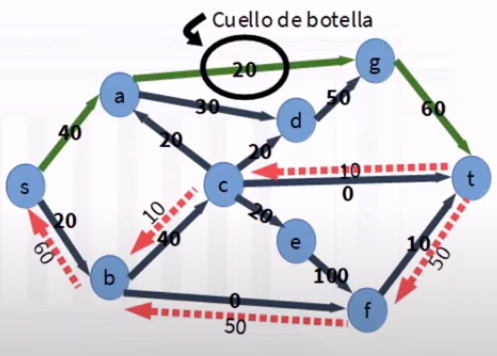
\includegraphics[width=\linewidth]{imagenes/cuello-de-botella.png}
\end{figure}

Lo máximo que se puede transportar es 20, para que no deje cumplir la condición de capacidad.

\begin{quote}
    \textit{Con el grafo residual, podemos redireccionar el flujo en el camino original para aumentar el flujo total de la red.}
\end{quote}

Tambien nos ayuda a saber cuanto flujo se esta trasportando por ese eje.

Llamamos \(P\) al camino de aumento (\textbf{augmenting path}):

\begin{itemize}
    \item \(P\) es una caminio simple que va de \(s\) a \(t\) en \(G_f\).
    \item \(P\) no visita el mismo nodo mas de una vez.
\end{itemize}
 
Ahora definimos la operación \textbf{augment(f,P)} el cual cede un nuevo flujo \(f'\) en e\(G\)

\begin{lstlisting}[language=Python, caption=Operación de augment]
augment(f, p)
    Sea b = bottleneck(P, f)
    Para cada eje e=(u, v) perteneciente a P
        Si e=(u,v) eje hacia adelante
            f(e) += b en G
        sino si es eje para atras 
            e' = (v,u)
            f(e') -=b en G   
    Retornar f
\end{lstlisting}


\begin{figure}[h!]
    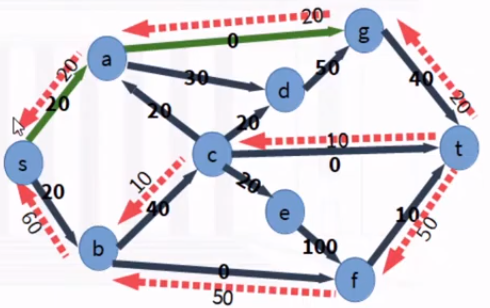
\includegraphics[width=\linewidth]{imagenes/camino-aumento.png}
\end{figure}

\textit{¿Es valido el nuevo flujo?}PENDIENTE

Con el grafo residual y el camino de aumento definimos el \textit{pseudocódigo de Ford-Fulkerson}.


\begin{lstlisting}[language=Python, caption=Operación de augment]
Max-Flow
    Inicialmente  f(e)=0 para todo 'e' en G

    Mientras haya un camino s-t en Gf

        Sea P un caminio s-t simple en Gf
        f' = augment(f,P)

        Actualizar f para ser f'
        Actualizar Gf para ser Gf'


    Retornar f
\end{lstlisting}

La \textbf{complejidad} es \(O(|E|*C)\) donde \(|E|\) es la cantidad de ejes y C es la suma de todas
las \(C_e\) de los ejes que salen de la fuente.


\textit{¿Es óptimo?}PENDIENTE

\begin{quote}
    \textbf{El flujo retornado por el algoritmo Ford-Fulkerson es el flujo máximo}
\end{quote}

Ademas podemos mediante BFS en \(G_f\) construir el corte mínimo s-t (A,B) obteniendo A y por diferencia B.

Consideraciones si las capacidades no son enteras:
\begin{itemize}
    \item Si son racionales, multiplicar por minimo comun multiplo
    \item Si son irracionales, \textit{no esta asegurado que el algoritmo termine}.
\end{itemize}

\subsection{Variante: Circulación con demanda}

Cada nodo pueder ser productor o consumir de flujo. O un nodo que no es consumidor ni productor de flujo.

\newpage
\subsection{Bipartite Matching Problem}

Llamamos un grafo bipartito a \(G=(V,E)\) un \textit{grafo no dirigido}, puede particionarse en 
como \(V=X \cup Y\), con la propiedad de que cada eje \(e \in E\) se conecta en una punta con
un nodo en \(X\) y la otra punta un nodo en \(Y\). Un \textit{matching M} en \(G\) es un subconjunto
de ejes \(M \subseteq E\) tal que cada nodo aparece en al menos un eje en \(M\).
Se necesita encontrar el set \(M\) de mayor tamaño posible. O sea la mayor cantidad de parejas.


Resolvemos el matching utilizando el problema de flujo máximo.
Construimos una red de flujo \(G'\) como la siguiente imagen. Pasamos todos los ejes a ejes dirigidos de
\(X\) a \(Y\). Luego agregamos el nodo \(s\) y un eje \((s,x)\) desde \(s\) a cada nodo en \(X\). 
Tambien agregamos el nodo \(t\) y un eje \((y,t)\) desde cada nodo en \(Y\) a \(t\).
Finalmente, le damos una capacidad de \(1\) a cada eje en \(G'\)

\begin{figure}[h!]
    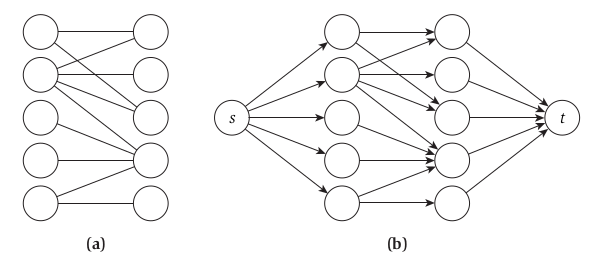
\includegraphics[width=\linewidth]{imagenes/bipartito-redes-flujo.png}
\end{figure}

Resolvemos el problema de red de flujo máximo con \(G'\). Obtenemos el flujo máximo \(s-t\). Entonces
\textit{El valor del flujo total es igual al tamaño del matiching máximo.}

\textbf{Analisis} Pendiente

\newpage
\subsection{Diseño de encuentas}

Considere el problema de una compañia que vende \(k\) productos y que tiene una base de datos con el 
historias de las compras de todos sus clientes. La compañia desea enviar encuestas con preguntas
personalizadas a un grupo particular de \(n\) clientes, para determinar que productos la gente 
prefiere sobre el total.

Lineamientos para la encuesta:
\begin{itemize}
    \item Cada cliente recibira preguntas acerca de cierto subconjunto de productos.
    \item Un cliente solo puede contestar sobre los productos que él o ella haya comprado.
    \item Cada cliente sera preguntado sobre un número de productos entre \(c_i\) y\(c'_i\) 
    \item Cada producto debe tener entre \(p_j\) y \(p'_j\) preguntas de clientes distintos.
\end{itemize}

El problema de diseño de encuentas toma como input un \textit{grafo bipartito} \(G\) cuyos nodos son 
clientes y productos, y hay un eje entre un cliente \(i\) y un producto \(j\) si el cliente compro el producto \(j\).
Mas aún, por cada cliente \(i=1,2,...,n\) tenemos la limitante de \(c_i \leq c'_i\) en el numero de productos en el que un 
cliente puede constestar; por cada producto \(j=1,...,k\), tenemos la limitante \(p_j \leq p'_j\) en el 
número de cliente distintos que se pueden consultar por cada producto.

\begin{figure}[h!]
    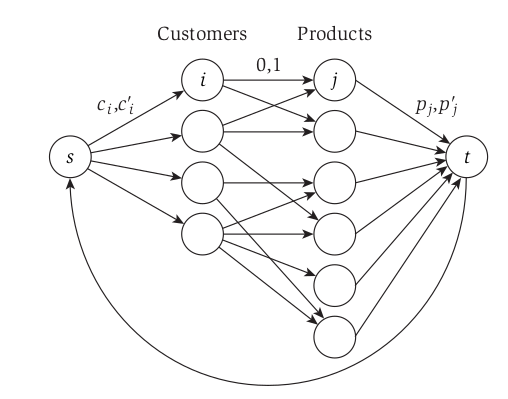
\includegraphics[width=\linewidth]{imagenes/grafo-encuesta.png}
\end{figure}

El problema se resuelve reduciendo este a un problema de red de flujo en \(G'\) con demanda y un limite inferior. 

Para obtener un grafo \(G'\) de \(G\), necesitamos:
\begin{itemize}
    \item Orientar los ejes de \(G\) desde los clientes a los productos.
    \item Agregar un nodo ficticio \(s\) con los ejes \((s,i)\) por cada cliente \(i=1,...,n\).
    \item Agragar un nodo ficticio \(t\) con los ejes \((j,t)\) por cada producto \(j=1,...,k\).
\end{itemize}

La circulacion en la red, corresponde con la manera en la que se tienen que realizar las preguntas.

Se debe pasar de un problema de circulación con \textit{demanda y limite inferior} a un problema
de circulación con demanda y luego a un problema de flujo máximo. Finalmente se resuelve con Ford-Fulkerson.

Una vez obtenido el flujo máximo:

\begin{itemize}
    \item El flujo que va de \((t,s)\) corresponde al número total de preguntas a realizar.
    \item El flujo en los ejes \((s,i)\) es el número de productos que deben contener el cuestionario para cada cliente \(i\).
    \item El flujo en los ejes \((j,t)\) corresponde con él numero de clientes que deben ser preguntados para el producto \(j\).
    \item Por ultimo, aquellos ejes \((i,j)\) con flujo 1, corresponden a preguntar al cliente \(i\) sobre el producto \(j\).
\end{itemize}

\newpage
\subsection{Problema de Selección de proyectos}

Dado un conjunto \(P\) de proyectos para seleccionar y cada proyecto \(i \in P\) tiene
asociado una ganancia \(p_i\), el cual puede ser \textit{positivo} como \textit{negativo}.
Algunos proyectos son requisitos de otros proyectos, y modelaremos esta relación mediante un \textit{grafo
dirigido sin ciclos} \(G=(P,E)\). Los nodos de \(G\) son los proyectos y hay un eje \((i,j)\) para indicar
que un proyecto \(i\) puede ser seleccionado solo si el proyecto \(j\) es tambien seleccionado.
Un proyecto \(i\) pude tener muchos prerequisitos, y puede haber muchos proyectos \(j\) que pueden
ser parte de esos prerequisitos. Un conjunto de proyecto de \(A \subseteq P\) es \textit{viable} si los 
prerequisitos de cada proyecto de \(A\) tambien pertenecen a \(A\):
\begin{quote}
    Por cada \(i \in A\) y cada eje \((i,j) \in E\), tenemos que \(j \in A\)
\end{quote}
Estos prerequisitos vendrian a ser las \textit{restricciones de precedencia}. La ganancia del conjunto de proyectos
se define como:

\[
    profit(A) = \sum_{i\in A} p_i 
\]

El \textit{problema de selección de proyectos} seleccionar el conjunto de proyectos viables con la maxima ganancia.



\end{document}





